\newpage

\section{Вычислительный эксперимент}

Для анализа моделей, полученных путем дистилляции модели учителя в модель ученика, проводится вычислительный эксперимент для задачи классификации.\\
Эксперимент проводится для выборки FashionMNIST~\cite{FMNIST} - набора изображений предметов одежды. В качестве моделей учителя $\textbf{f}$ и ученика $\textbf{g}$ рассматриваются четырёхслойная и однослойная нейронные сети соответсвенно. Для решения оптимизационной задачи используется Adam, функция активации - ReLu.\\
Выборка разделяется на 3 части: две для обучения многоресурного и малоресурсного доменов, а также тестовая часть выборки. Многоресурсная часть содержит 59000 объектов, малоресурсная часть содержит 1000 объектов, а тестовая часть содержит 10000 объектов.

\subsection{Анализ дистилляции Хинтона}

\paragraph{Обучение на обоих доменах.}
Модели учителя и ученика обучаются на обоих доменах.\\
\begin{figure}[h!t]\center
\subfloat[]
{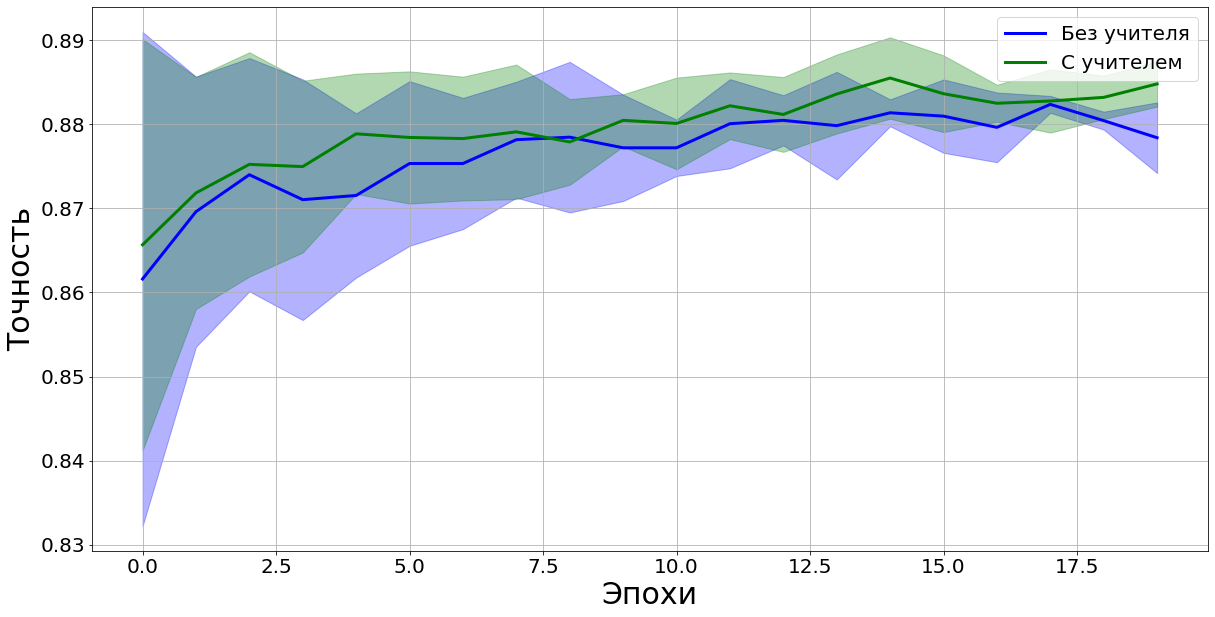
\includegraphics[width=0.5\textwidth]{results/acc}}
\subfloat[]
{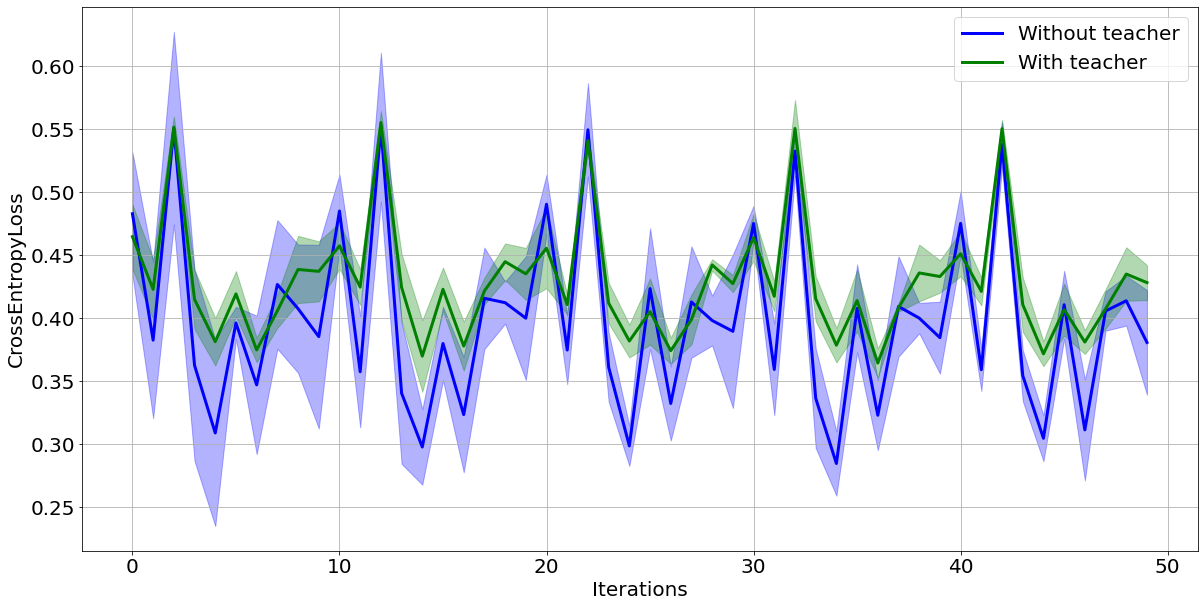
\includegraphics[width=0.5\textwidth]{results/loss}}\\
\caption{Качество аппроксимации на тестовой выборке a) accuracy; b) CrossEntropyLoss между истинными и предсказанными учеником метками}
\end{figure}\\
На рис.1а показан график зависимости метрики accuracy на тестовой выборке между истинными метками объектов и вероятностями, предсказанными моделью ученика.\\
На рис.1б показан график зависимости кросс-энтропии на тестовой выборке между истинными метками объектов и вероятностями, предсказанными моделью ученика.\\
На графиках видно, что модель, использующая метки учителя, показывает лучшее значение accuracy, при этом наблюдается значительное снижение ошибки.


\paragraph{Обучение на малоресурсном домене.}
Модель учителя обучается на многоресурсном домене, а модель ученика обучается на малоресурсном домене.\\
\begin{figure}[h!t]\center
\subfloat[]
{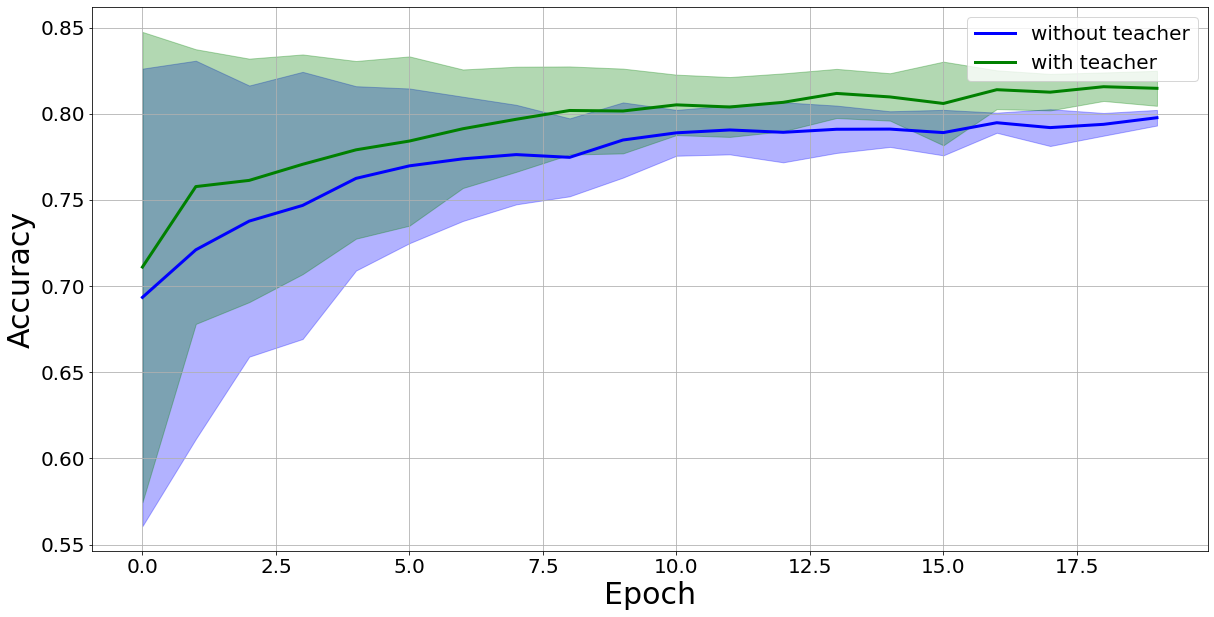
\includegraphics[width=0.5\textwidth]{results/small_acc}}
\subfloat[]
{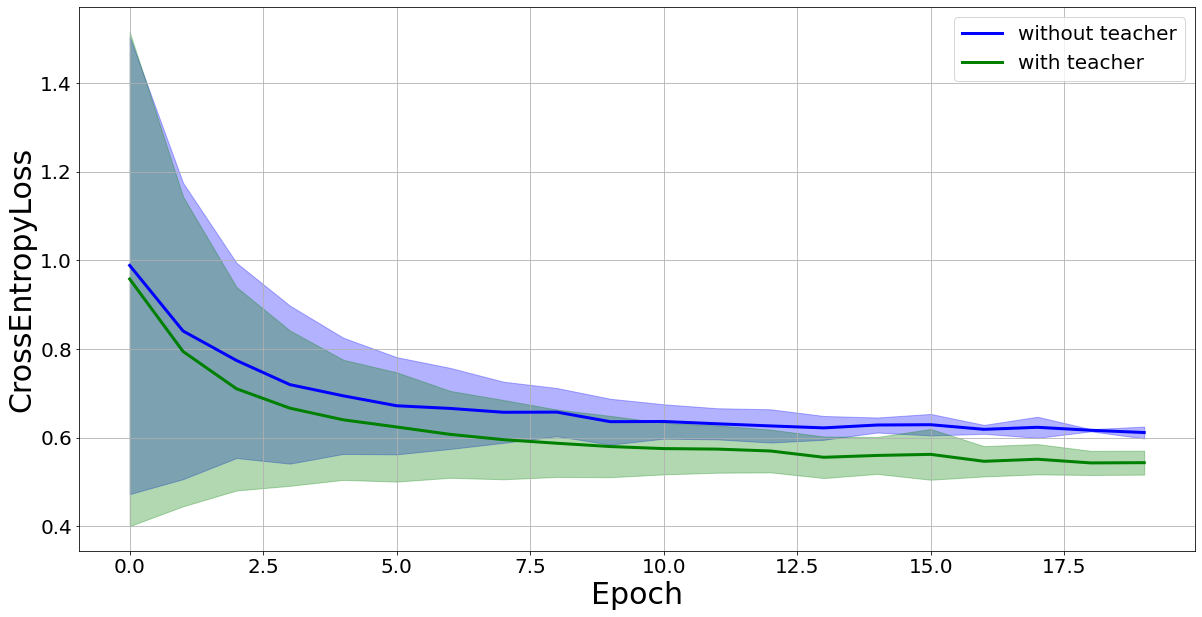
\includegraphics[width=0.5\textwidth]{results/small_loss}}\\
\caption{Качество аппроксимации на тестовой выборке a) accuracy; b) CrossEntropyLoss между истинными и предсказанными учеником метками}
\end{figure}\\
На рис.2а показан график зависимости метрики accuracy на тестовой выборке между истинными метками объектов и вероятностями, предсказанными моделью ученика.\\
На рис.2б показан график зависимости кросс-энтропии на тестовой выборке между истинными метками объектов и вероятностями, предсказанными моделью ученика.\\
На графиках видно, что модель, использующая метки учителя, показывает лучшее значение accuracy, при этом наблюдается снижение ошибки.

\newpage
\paragraph{Обучение на выборке с шумом.}
Добавим к многоресурсному домену нормальный шум $\mathcal{N}(0,0.1)$ и обучим на нем модель учителя. Модель ученика обучается на малоресурсном домене.
\begin{figure}[h!t]\center
{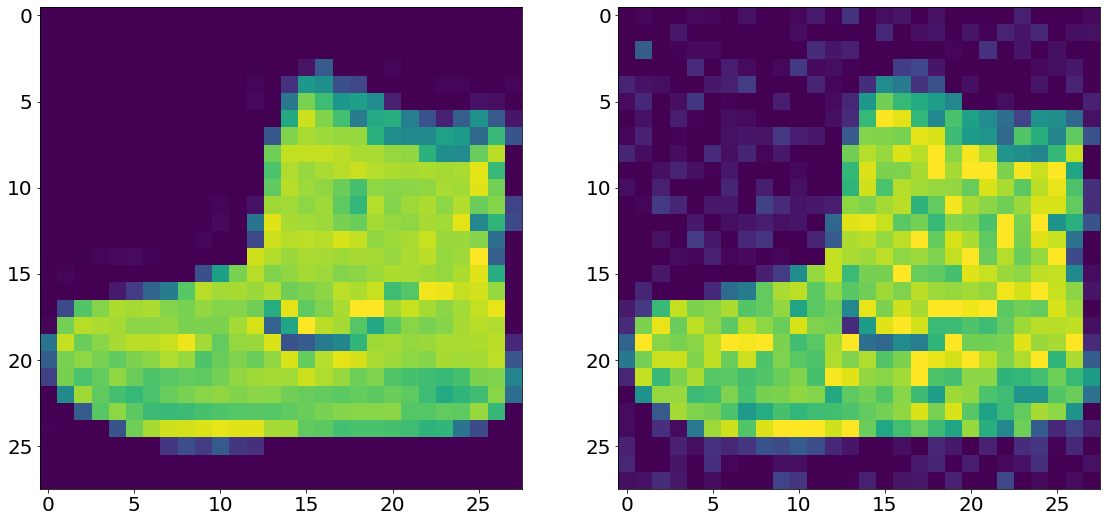
\includegraphics[width=0.5\textwidth]{results/noise}}
\caption{Сравнение объекта выборки до и после добавления шума}
\end{figure}\\

\begin{figure}[h!t]\center
\subfloat[]
{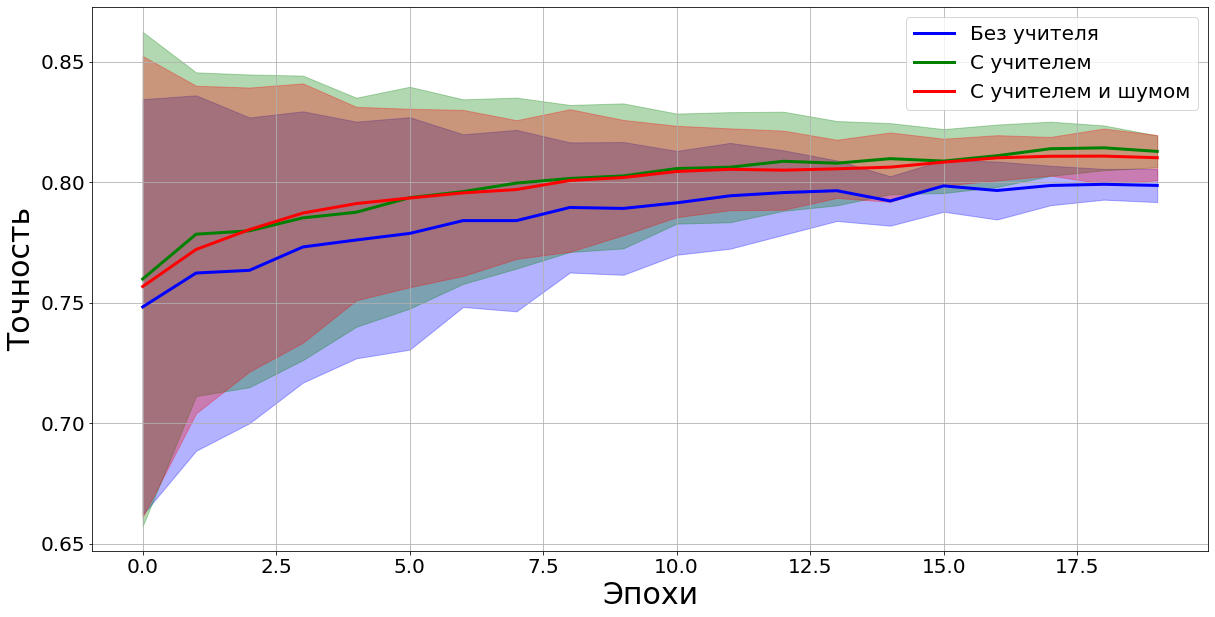
\includegraphics[width=0.5\textwidth]{results/noise_acc}}
\subfloat[]
{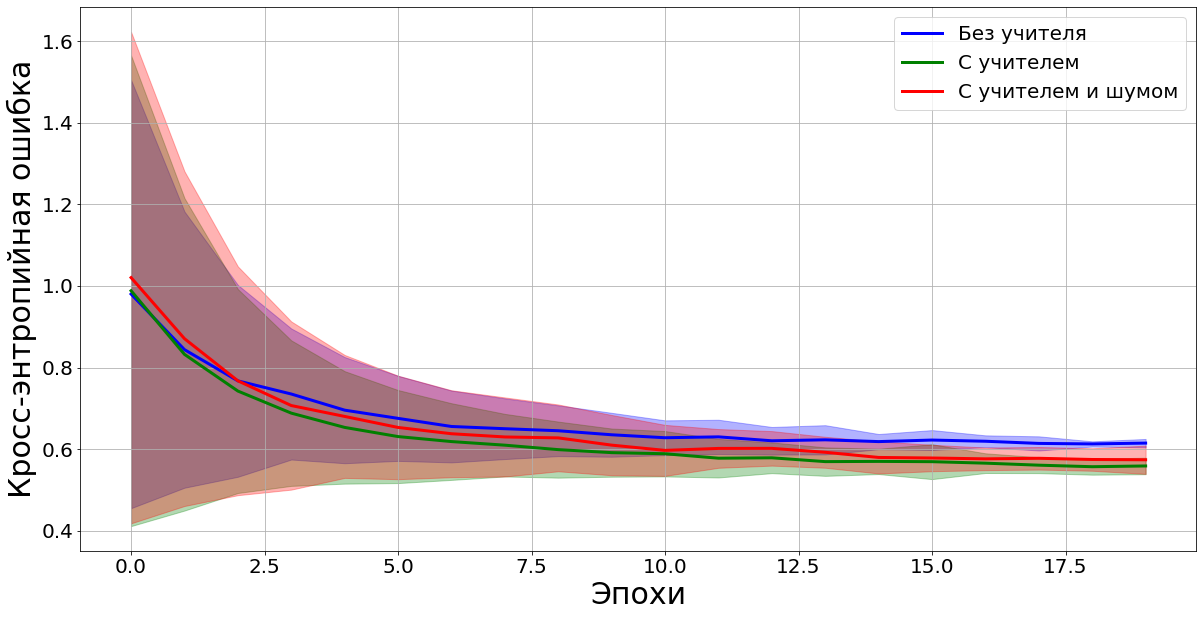
\includegraphics[width=0.5\textwidth]{results/noise_loss}}\\
\caption{Качество аппроксимации на тестовой выборке a) accuracy; b) CrossEntropyLoss между истинными и предсказанными учеником метками}
\end{figure}\\
На рис.4а показан график зависимости метрики accuracy на тестовой выборке между истинными метками объектов и вероятностями, предсказанными моделью ученика.\\
На рис.4б показан график зависимости кросс-энтропии на тестовой выборке между истинными метками объектов и вероятностями, предсказанными моделью ученика.\\
На графиках видно, что значения accuracy и CrossEntropyLoss модели, использующей метки учителя на выборке с шумом, лежат между соответствующими значениями для модели без учителя и для модели, использующей метки учителя на выборке без шума.

\paragraph{Обучение на выборке с dilation.}
Применим к многоресурсному домену сверточное преобразование с параметром $\text{dilation}=2$ и обучим на нем модель учителя. Модель ученика обучается на малоресурсном домене.\\
\begin{figure}[h!t]\center
{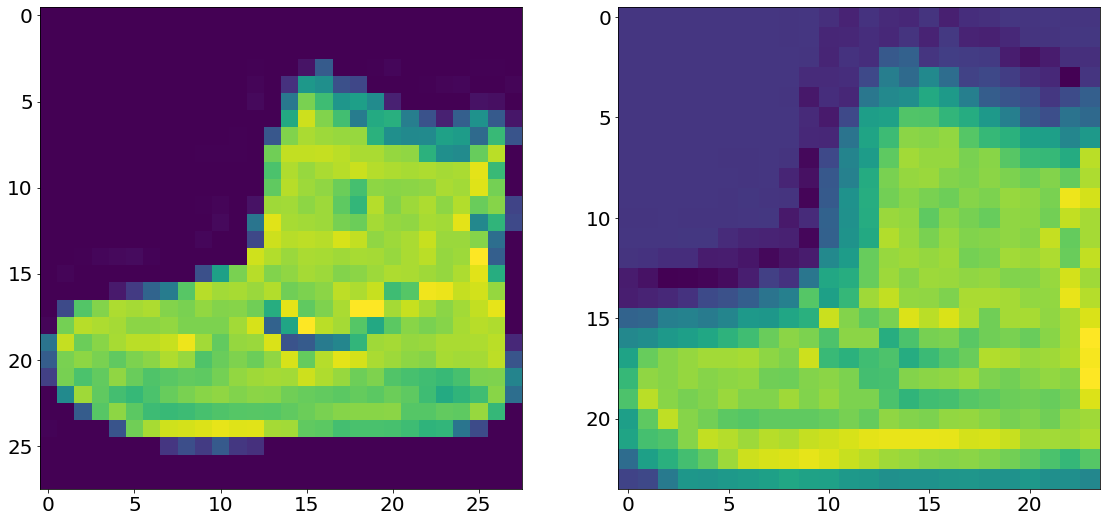
\includegraphics[width=0.5\textwidth]{results/dilation}}
\caption{Сравнение объекта выборки до и после преобразования}
\end{figure}\\

\begin{figure}[h!t]\center
\subfloat[]
{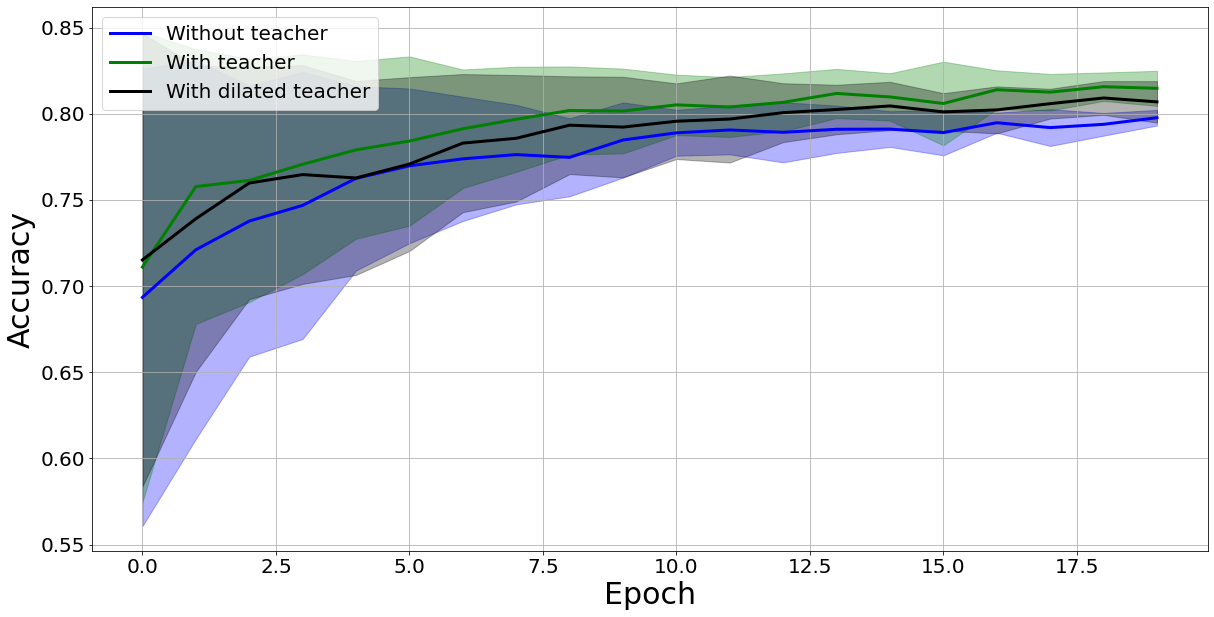
\includegraphics[width=0.5\textwidth]{results/dilation_acc}}
\subfloat[]
{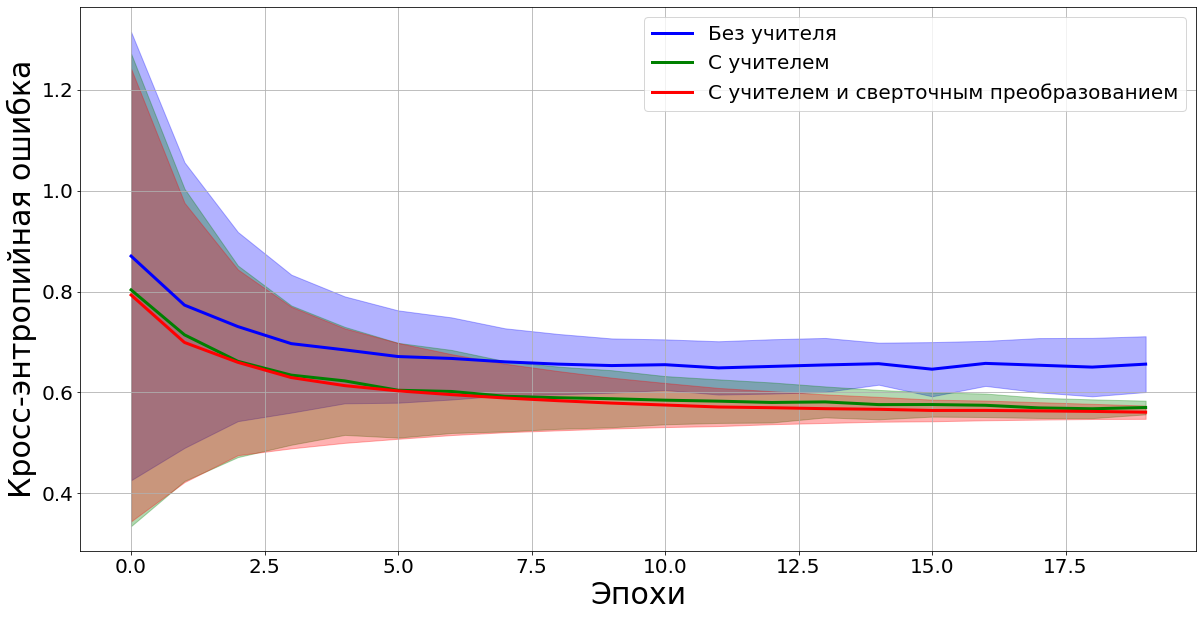
\includegraphics[width=0.5\textwidth]{results/dilation_loss}}\\
\caption{Качество аппроксимации на тестовой выборке a) accuracy; b) CrossEntropyLoss между истинными и предсказанными учеником метками}
\end{figure}\\
На рис.6а показан график зависимости метрики accuracy на тестовой выборке между истинными метками объектов и вероятностями, предсказанными моделью ученика.\\
На рис.6б показан график зависимости кросс-энтропии на тестовой выборке между истинными метками объектов и вероятностями, предсказанными моделью ученика.\\
На графиках видно, что значения accuracy и CrossEntropyLoss модели, использующей метки учителя на выборке с преобразованием, лежат между соответствующими значениями для модели без учителя и для модели, использующей метки учителя на выборке без преобразования.

\subsection{Вариационный автокодировщик}
В качестве преобразования выборки FashionMNIST~\cite{FMNIST} будем использовать модель вариационного автокодировщика. Данная модель состоит из двух частей. Сначала строится вероятностоное распределение в скрытом пространстве, которое позволяет генерировать кодовые представления для одного объекта. Далее с помощью декодировщика строится вероятностное распределение, позволяющее генерировать реконструкци исходного объекта.\\
\\
$\mathbf{q_{\alpha}(z|x)}$-вероятностный кодировщик\\
$\mathbf{p_{\beta}(\hat{x}|z)}$-вероятностный декодировщик\\
$\mathbf{\mathcal{L}_{\text{VAE}}(\alpha, \beta)=\sum\limits_{i=1}^{l}\text{E}_{z\sim q_{\alpha}(z|x_{i})}\log{p_{\beta}(x_{i}|z)}dz-\text{KL}(q_{\alpha}(z|x_{i})||p(z))}$,\\
\\
$\mathbf{p(z)\sim \mathcal{N}(0,\sigma^{2}\mathbf{I})}$ - априорное распределение\\
\\
Получаем оптимизационную задачу:
$$\hat{\alpha}, \hat{\beta} = \arg\max_{\alpha, \beta} \mathcal{L}(\alpha, \beta).$$

\newpage
\subsection{Генерация отображения из FashionMNIST в MNIST}
Воспользуемся моделью вариационного автокодировщика для преобразования изображений одежды из выборки FashionMNIST~\cite{FMNIST} в изображения цифр на основе выборки MNIST.\\
Создадим синтетическую выборку, где каждому изображению одежды будет соответстовать случайное изображение цифры из того же класса.\\
\begin{figure}[h!t]\center
\subfloat[]
{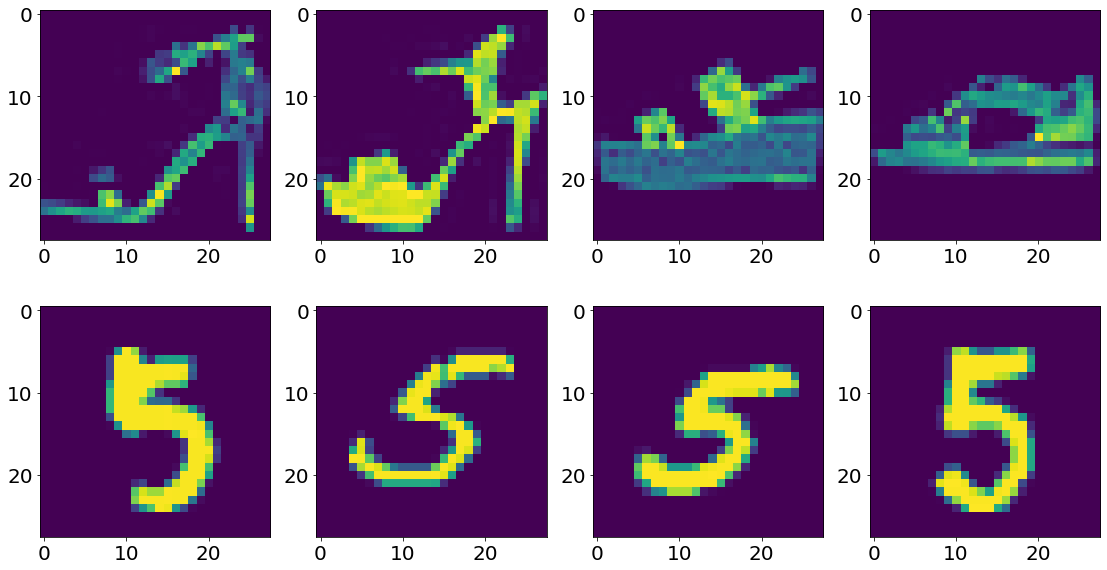
\includegraphics[width=0.5\textwidth]{results/fmnist_random_mnist.png}}
\subfloat[]
{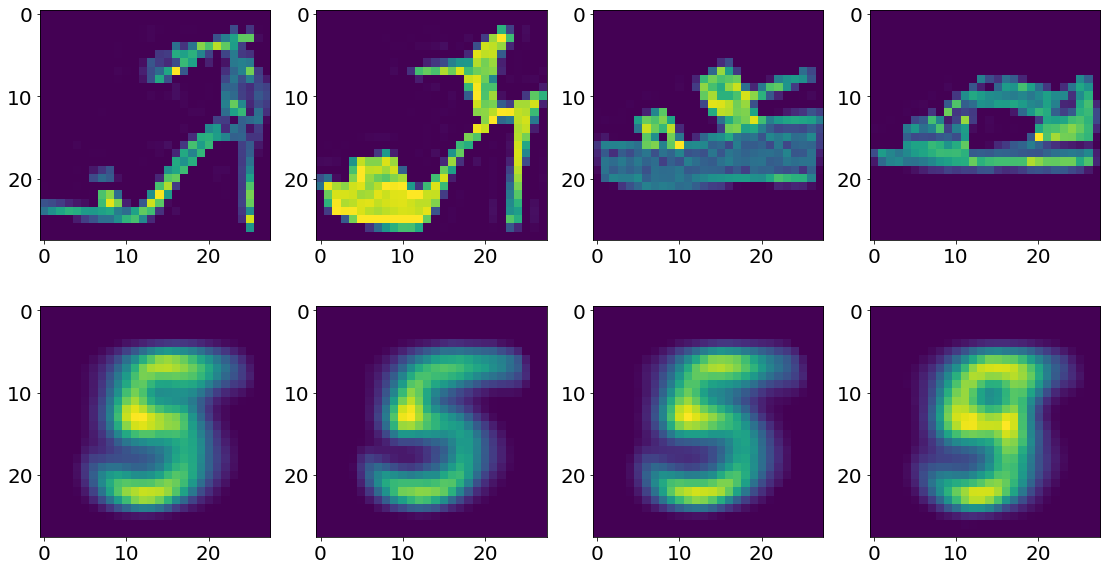
\includegraphics[width=0.5\textwidth]{results/fmnist_vae_mnist.png}}\\
\caption{a) Объекты синтетический выборки; b) Объекты исходной выборки до и после работы автокодировщика}
\end{figure}\\
Далее, на основе данной выборки обучим модель вариационного автокодировщика, минимизируя ошибку между выходом модели и целевым значением - изображением цифры, соответствующего исходному объекту.\\
Получили модель, генерирующую семейство новых объектов - изображений цифры для одного и того же изображения одежды.
\newpage
Посмотрим также на изменение выхода модели при изменении случайного вектора в скрытом представлении:\\
\begin{figure}[h!t]\center
{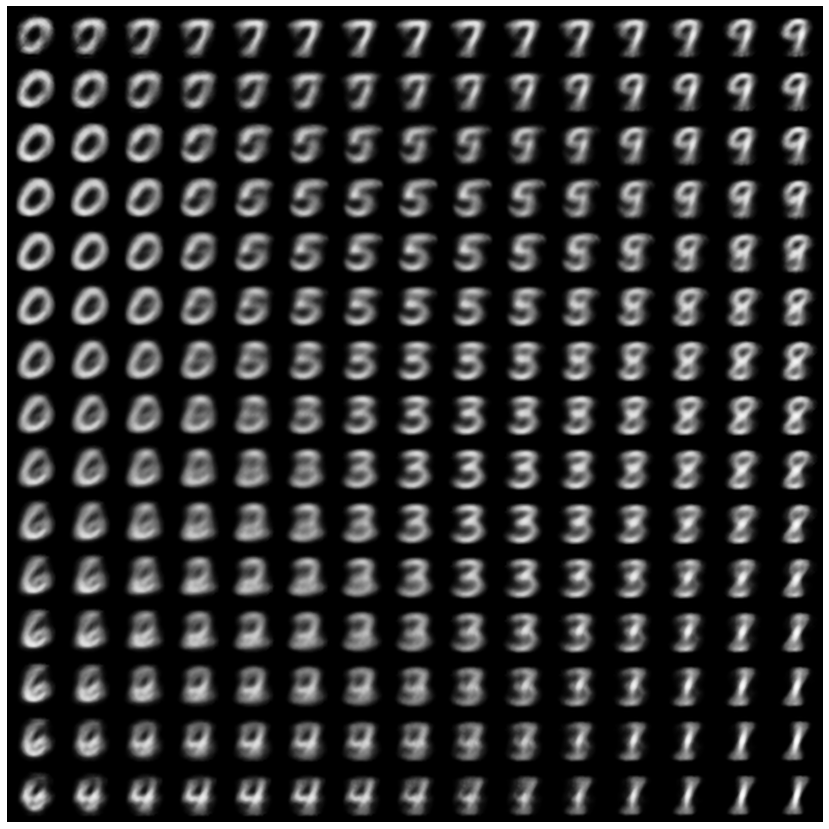
\includegraphics[width=0.5\textwidth]{results/10x10.png}}
\caption{Зависимость выхода модели от изменения вектора в скрытом представлении}
\end{figure}\\

\subsection{Качество модели в зависимости от использования автокодировщика}
Будем обучать модель учителя на выборке MNIST, а модель ученика на выборке FashionMNIST. При этом при обучении модели ученика будем использовать метки учителя, подавая ему на вход выход вариационного автокодировщика, переводящего изображения одежды в изображения цифр.\\
\begin{figure}[h!t]\center
\subfloat[]
{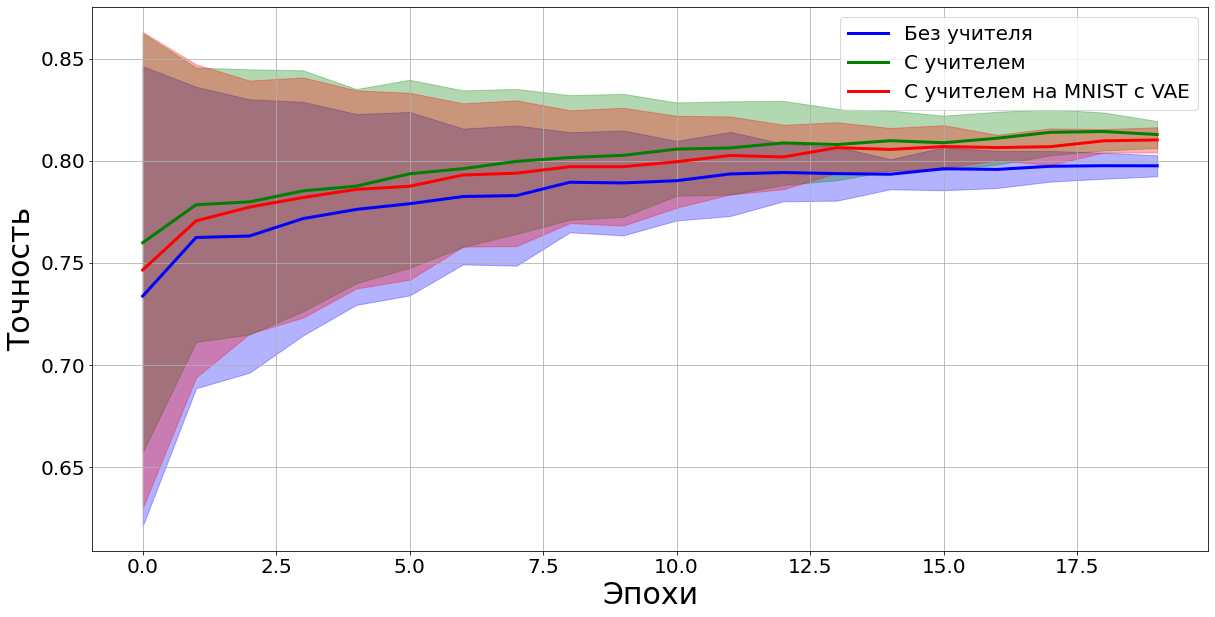
\includegraphics[width=0.5\textwidth]{results/vae_acc}}
\subfloat[]
{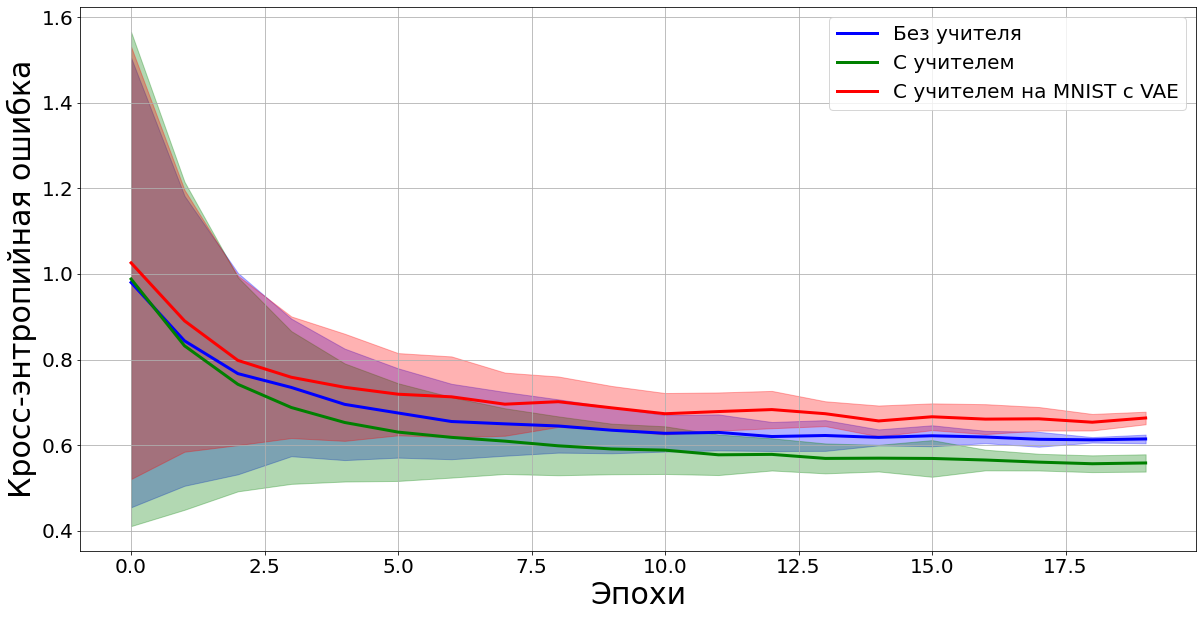
\includegraphics[width=0.5\textwidth]{results/vae_loss}}\\
\caption{Качество аппроксимации при использовании VAE на малодоменной выборке a) accuracy; b) CrossEntropyLoss между истинными и предсказанными учеником метками}
\end{figure}\\
Также для сравнения покажем качество аппроксимации без использования вариационного автокодировщика.\\
\begin{figure}[h!t]\center
\subfloat[]
{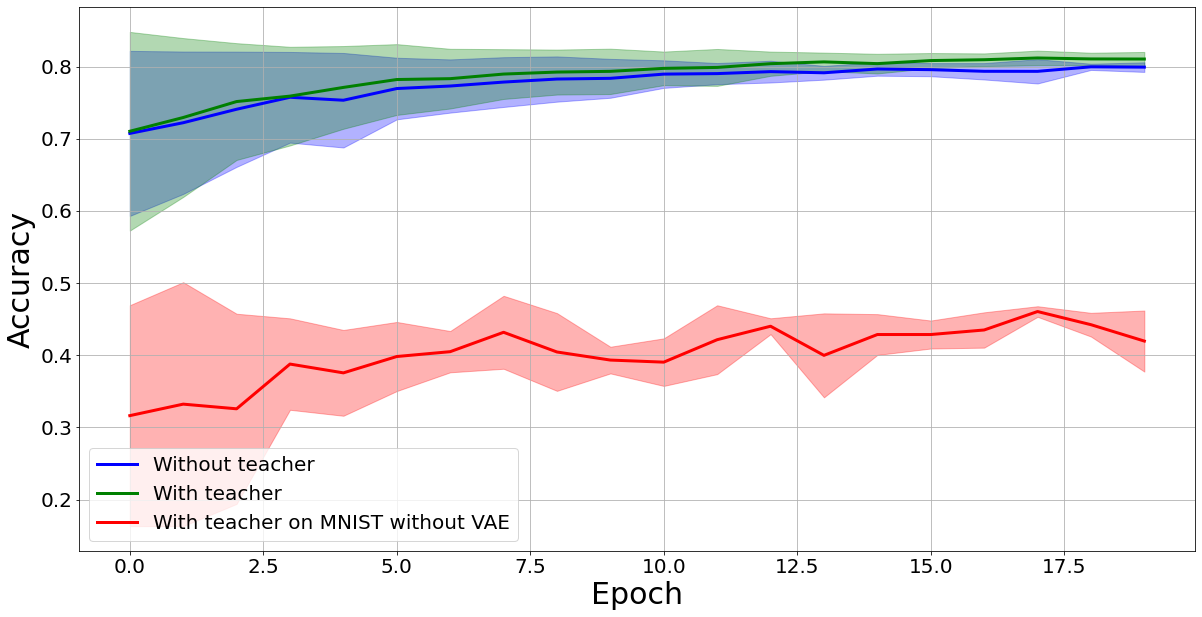
\includegraphics[width=0.5\textwidth]{results/mnist_acc}}
\subfloat[]
{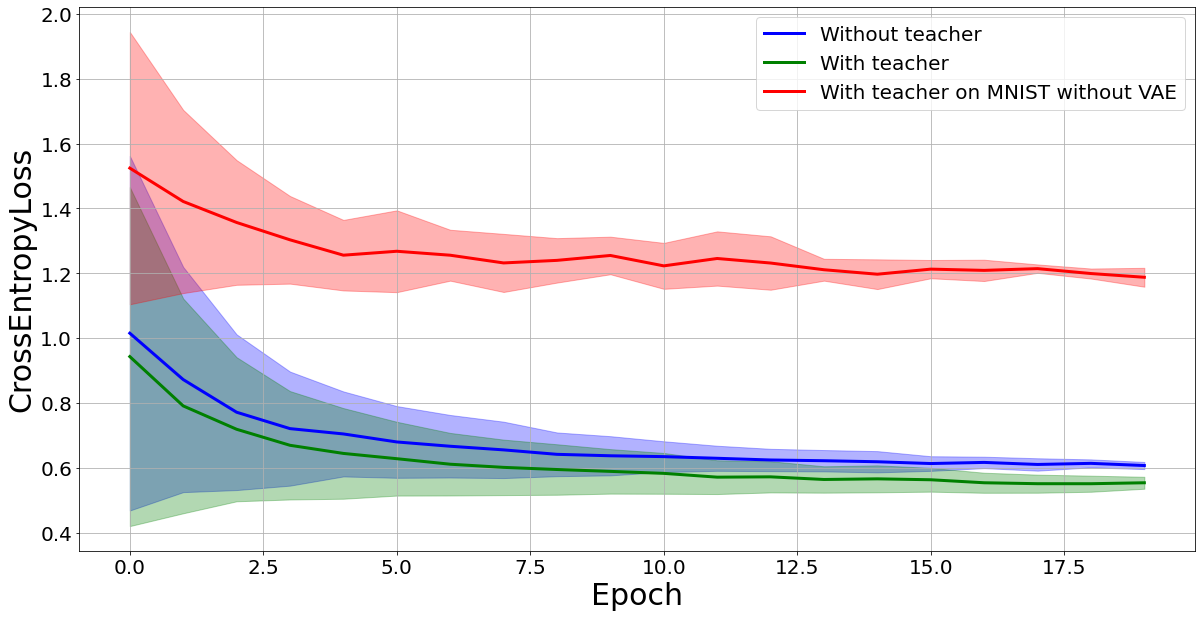
\includegraphics[width=0.5\textwidth]{results/mnist_loss}}\\
\caption{Качество аппроксимации без использования VAE на малодоменной выборке a) accuracy; b) CrossEntropyLoss между истинными и предсказанными учеником метками}
\end{figure}

\newpage
\subsection{Качество модели на сгенерированной выборке}
Для каждого объекта малодоменной выборки сгенерируем 70 изображений цифр с помощью модели вариационного автокодировщика и создадим новую выборку из 70000 объектов.\\
Модель ученика обучается на малодоменной выборке, модель учителя на новой выборке и используется при обучении ученика.